\documentclass[12pt]{report}
\usepackage[english]{babel}
\usepackage[utf8x]{inputenc}
\usepackage{amsmath}
\usepackage{graphicx}
\usepackage[colorinlistoftodos]{todonotes}
\usepackage[left=2cm,right=2cm,top=2.5cm,bottom=2cm]{geometry}
\usepackage[]{algorithm2e}
\usepackage{amsmath}
\usepackage{amssymb}

\begin{document}

%----------------------------------------------------------------------------------------
%	MAIN PAGE
%----------------------------------------------------------------------------------------
\begin{titlepage}
\vspace*{\fill}
\newcommand{\HRule}{\rule{\linewidth}{0.5mm}}

\center

\textsc{\LARGE Aix-Marseille Université}\\[1.5cm]
\textsc{\Large Compléxité}\\[0.5cm]

\HRule \\[0.4cm]
{ \huge \bfseries Le Solveur Minisat}\\[0.4cm] % Title of your document
\HRule \\[1.5cm]

\begin{minipage}{0.4\textwidth}
\begin{flushleft} \large
\emph{Autheur:}\\
Michaël \textsc{Gileta} \\
Yohan \textsc{Roux}
\end{flushleft}
\end{minipage}
~
\begin{minipage}{0.4\textwidth}
\begin{flushright} \large
\emph{Référent:} \\
Kévin \textsc{Perrot}
\end{flushright}
\end{minipage}\\[2cm]

{\large Vendredi 13 Octobre}\\[2cm]


\includegraphics[scale=0.5]{./images/logo.png}\\[1cm]

\vspace*{\fill}
\end{titlepage}

%----------------------------------------------------------------------------------------

\section*{Exercice 1}
\subsection*{Question a}
(A OR B OR NOT(C) OR D) \\
AND\\
(NOT(B) OR C)\\
AND\\
(NOT (A) OR NOT (D))

\subsection*{Question b}
\subsubsection*{Conversion format intermédiaire}
$( 1\| 2 \| -3 \| 4 )$\\
\& \\
$( -2 \| 3 )$\\
\& \\
$( -1 \| -4 )$
\subsubsection*{Conversion format Minisat}
p cnf 4 3\\
1 2 -3 4 0\\
-2 3 0\\
-1 -4 0
\subsubsection*{Réponse Minisat}
La formule est satisfaisable.

\subsection*{Question c}
\subsubsection*{i.}
$\Phi = (\lnot t \rightarrow \lnot s) \rightarrow (((b \lor t) \rightarrow s) \land ((r \land m) \rightarrow (b \lor a))\land \lnot r)$ 
\begin{enumerate}
	\item $(t \lor \lnot s) \equiv (\lnot t \rightarrow \lnot s)$
	\item $(b \lor t) \rightarrow s \equiv (\lnot b \land \lnot t) \lor s \equiv (s\lor \lnot b) \land (s \lor \lnot t)$
	\item $(r \land m) \rightarrow (b \lor a) \equiv (\lnot r \lor \lnot m) \lor (b \lor a) \equiv (\lnot r \lor \lnot m \lor b \lor a)$
\end{enumerate}
$\Phi_2 = (t \lor \lnot s) \rightarrow ((s \lor \lnot b) \land (s \lor \lnot t) \land (\lnot r \lor \lnot m \lor b \lor a) \land \lnot r)$

$= (\lnot t \land s) \lor ((s \lor \lnot b) \land (s\lor \lnot t) \land (\lnot r \lor \lnot m \lor b \lor a) \land \lnot r)$

$= (\lnot t \lor s \lor \lnot b) \land (\lnot t \lor s) \land (\lnot t \lor \lnot r \lor \lnot m \lor b \lor a) \land (\lnot r \lor \lnot t) \land (s \lor \lnot b) \land (s \lor \lnot t) \land (s \lor \lnot r \lor \lnot m \lor b \lor a) \land (\lnot r \lor s)$

$= (\lnot t \lor s \lor \lnot b) \land (\lnot t \lor s) \land (\lnot t \lor \lnot r \lor \lnot m \lor b \lor a) \land (\lnot r \lor \lnot t) \land (s \lor \lnot b) \land (s \lor \lnot r \lor \lnot m \lor b \lor a) \land (s \lor \lnot r)$

\subsubsection*{ii.}
(NOT(T) OR S OR NOT(B) ) \\
AND \\
(NOT(T) OR S ) \\
AND \\
(NOT(T) OR NOT(R) OR NOT(M) OR B OR A ) \\
AND \\
(NOT(R) OR NOT(T) ) \\
AND \\
(S OR NOT(B) ) \\
AND \\
(S OR NOT(R) OR NOT(M) OR B OR A ) \\
AND \\
(S OR NOT(R) )

\subsubsection*{iii.}
p cnf 6 8\\
-1 2 -4 0\\
-1 2 0\\
-1-5 -6 4 3 0\\
-5 -1 0\\
2 -4 0
2 -5 -6 4 3 0\\
2 -5 0\\

\noindent Correspondance entre les numéros des variables et leur significations. \\
T = 1, S = 2, A = 3, B = 4, R = 5, M = 6 \\
Lors de la première exécution, la formule est satisfaisable avec ce résultat : -1 -2 -3 -4 -5 -6 0 \\
Ce qui correspond à l'affectation des valeurs correspondantes : \\
T = 0, S = 0, A = 0, B = 0, R = 0, M = 0 \\

\noindent Pour avoir une autre solution il suffit d'ajouter le négatif de la solution trouvé en premier lieu en clause. \\
Nouvelle clause ajouté à la fin du fichier:  1 2 3 4 5 6 0 \\
On obtient bien une autre solution: -1 2 -3 -4 -5 -6 0 \\
T = 0, S = 1, A = 0, B = 0, R = 0, M = 0 

\newpage
\subsection*{Question d}
\begin{algorithm}[H]
	Fonction Test \\
	Entrée : un nombre binaire i et $\Phi$ une formule. \\
	Sortie : SAT si $\Phi$ est Satisfaisable avec i comme modèle, INSAT sinon
\end{algorithm}

\begin{algorithm}[H]
	Fonction IsTautology \\
	Entrée : un nombre binaire i et $\Phi$ une formule. \\
	Sortie : SAT si $\Phi$ est Satisfaisable avec i comme modèle, INSAT sinon \\
	\Begin{
		b = $2^{NbVar}-1$
		\For{i : 0 $\rightarrow$ b}{
			\eIf{Test(bytes(i), $\Phi$)} {
				Retourne FAUX
			}{}
		}
		Retourne Vrai
	}
\end{algorithm}

\subsection*{Question e}
\subsubsection*{i.}
Un seul objet par tirroir : \\
$\rightarrow$ Soit $C_{i,j}$ l'objet i ($1<i<n+1$) dans le tirroir j ($1 < j < n$) \\
$\underset{i \rightarrow n+1}{\land} (\underset{j \rightarrow n}{\lor} C_{ij})$ \\

\noindent Un tirroir ne peut avoir qu'un seul objet : \\
$\underset{i \rightarrow n+1}{\land} (\underset{i \rightarrow n+1}{\lor} (C_{ij} \overset{k \rightarrow n+1}{\underset{i \neq k}{\land}} \lnot C_{kj})$ \\

\subsubsection*{ii.}
Test sur la valeur n=2, voir le fichier e.cnf

\subsubsection*{iii.}
Si l'on fait croitre n, le nombre de clause augmente de façon exponentiel.
\newpage
\section*{Exercice 2}
\begin{enumerate}
\item Soit une réduction polynomiale d'un problème 3-COL à SAT \\
Un sommet peut prendre 3 valeurs possibles, une par couleur soit RGB (Red, Green, Blue). \\
Ces valeurs sont évalué à 1 si le sommet a cette couleur, et à 0 sinon. \\
Soit R1,G1,B1, le triplet de valeur pour le sommet 1. \\

\noindent Pour chaque sommet, on obtient 4 clauses. \\
(R1 $\lor$ G1 $\lor$ B1) $\land$ ($\lnot$R1 $\lor$ $\lnot$G1) $\land$ ($\lnot$R1 $\lor$ $\lnot$B1) $\land$ ($\lnot$B1 $\lor$ $\lnot$G1)\\
Ces 4 clauses sont pour chaque sommet appartenant au graph.\\

\noindent Ensuite en fonction des arrêtes du graph, plusieurs clauses se forment. \\
Pour une arrête entre le sommet 1 et 2. On génére les 3 clauses suivantes. \\
($\lnot$R1 $\lor$ $\lnot$R2) $\land$ ($\lnot$G1 $\lor$ $\lnot$G2) $\land$ ($\lnot$B1 $\lor$ $\lnot$B2)\\
On génére donc ces 3 clauses pour chaque arrêtes du graphes. \\

\noindent On obtient donc : \\
$\underset{i \rightarrow nbSommet}{\land} (Ri \lor Gi \lor Bi) \land (\lnot Ri \lor \lnot Gi) \land (\lnot Ri \lor \lnot Bi) \land (\lnot Bi \lor \lnot Gi)$ \\
$\underset{i,j \rightarrow nbSommet}{\land} (\lnot Ri \lor \lnot Rj) \land (\lnot Gi \lor \lnot Gj) \land (\lnot Bi \lor \lnot Bj) $
\item Graph :\\
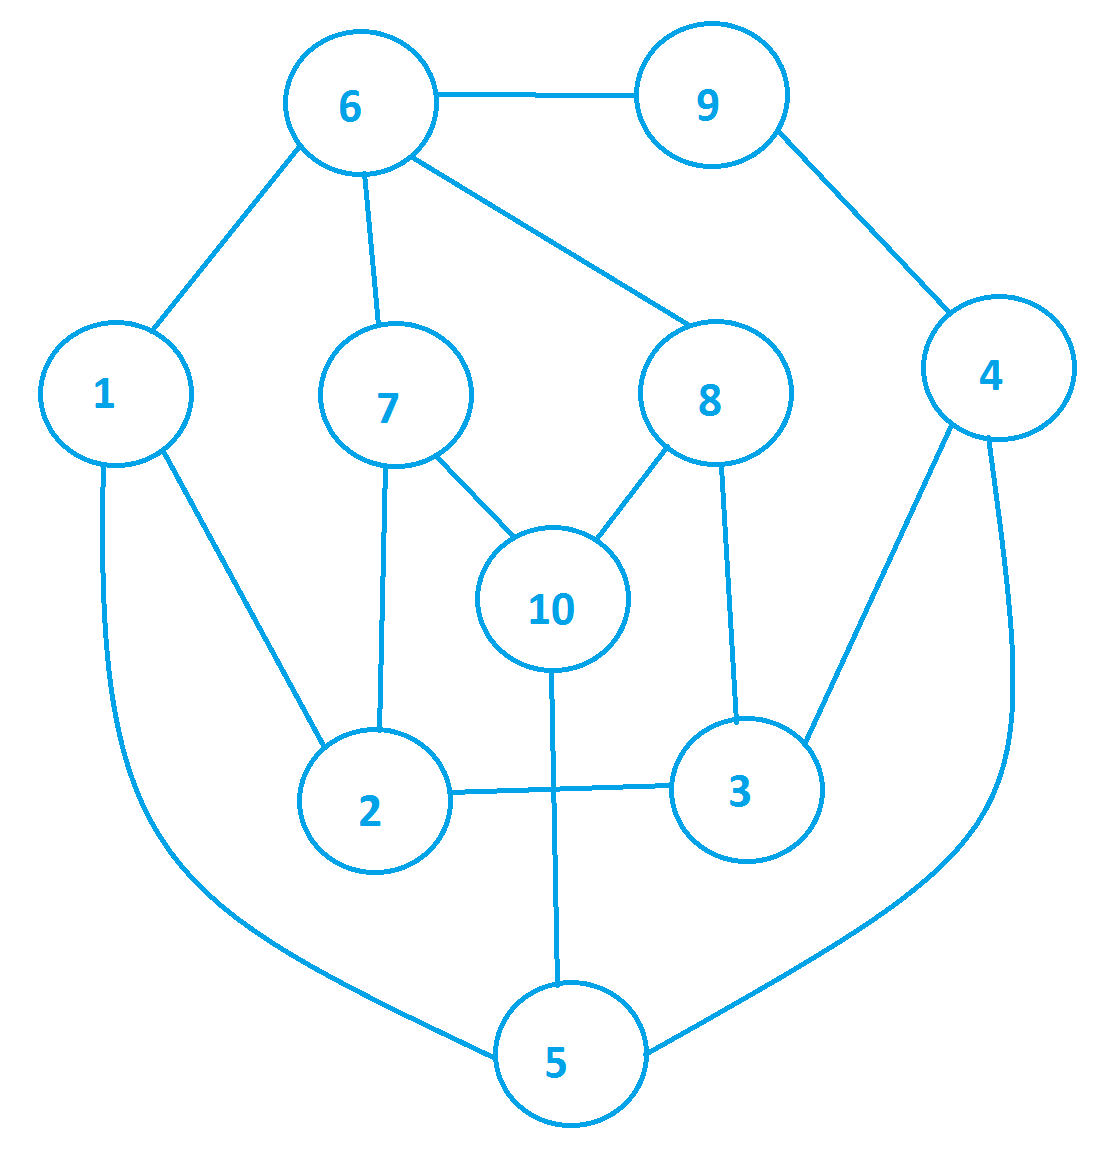
\includegraphics[scale=0.5]{./graph.png}\\[1cm]
\item Voir programme joint
\item Voir programme joint
\item Voir programme joint
\item Quand on fait grandir la taille du graph, le nombre de clause vaut : \\4xNbSommets + 3xNbArretes, ce qui se fait rapidement. \\
Mais le temps de résolution est de plus en plus long.
\end{enumerate}
\end{document}